\documentclass{article}
\usepackage{graphicx}
\usepackage{float}
\usepackage[a4paper, margin=2cm]{geometry}
\usepackage{titlesec}
\usepackage[font=small,labelfont=bf]{caption}
\usepackage{subcaption} % <— pour les sous-figures
\usepackage{booktabs}
\usepackage{siunitx}
\usepackage{tabularx}
\sisetup{
  detect-all,
  separate-uncertainty,
  table-number-alignment = center,
  table-figures-integer = 3,
  table-figures-decimal = 3
}

\titleformat{\section}{\normalfont\large\bfseries}{\thesection}{1em}{}
\titleformat{\subsection}[block]{\centering\normalfont\normalsize\bfseries}{}{0pt}{}

\title{Rapport}

% Chemin commun aux images
\graphicspath{{rapport_image_divers/}}

\begin{document}

\maketitle

\section*{Environnement :}

\section*{1er essai avec une asymétrie :}


\subsection{Paramètres :}
\begin{table}[H]
  \centering
  \caption{Paramètres de la simulation (issus de \texttt{param\_simu.py})}
  \label{tab:params}
  \begin{tabularx}{0.95\linewidth}{
      >{\raggedright\arraybackslash}p{4cm}
      >{\raggedright\arraybackslash}p{2.5cm}
      S[table-format=3.3]
      >{\raggedright\arraybackslash}X
  }
    \toprule
    \textbf{Symbole / Nom} & \textbf{Unité} & \textbf{Valeur} & \textbf{Description} \\
    \midrule
    Profondeurs puits 0       & \si{\milli\electronvolt} & (30, 5, 5, 40) & Énergies des 4 puits \\
    Profondeurs puits 1       & \si{\milli\electronvolt} & (30, 5, 5, 40) & Énergies des 4 puits \\
    Profondeurs puits  2      & \si{\milli\electronvolt} & (30, 5, 5, 40) & Énergies des 4 puits \\
    Hauteurs barrières       & \si{\milli\electronvolt} & (35, 90, 50) & Hauteurs des 3 barrières \\
    Hauteurs barrières       & \si{\milli\electronvolt} & (35, 90, 50) & Hauteurs des 3 barrières \\
    Hauteurs barrières       & \si{\milli\electronvolt} & (35, 90, 50) & Hauteurs des 3 barrières \\
    Largeur des puits        & \si{\nano\metre} & 23 & Largeur typique des puits \\
    Largeurs barrières       & \si{\nano\metre} & (15, 30, 25) & Largeurs des barrières \\
    \bottomrule
  \end{tabularx}
\end{table}


\section*{2ieme essai avec une asymétrie :}

% --- Figure avec deux sous-figures + une image pleine largeur ---
\begin{figure}[H]
  \centering
  \begin{subfigure}[c]{0.48\textwidth}
    \centering
    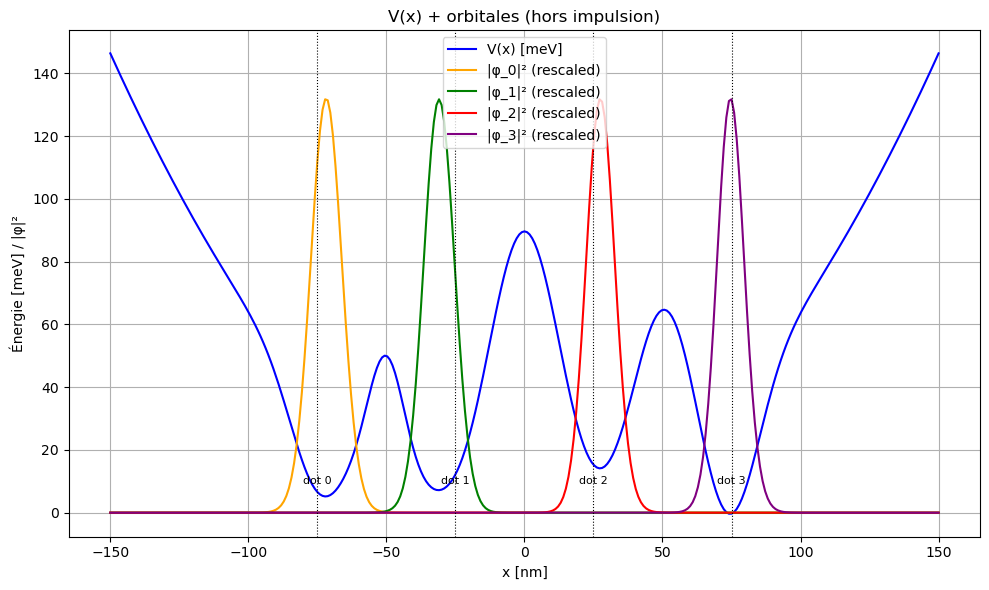
\includegraphics[width=\textwidth]{hors_impulsion_bon.png}
    \subcaption{Vue 1D hors impulsion}
    \label{fig:view_1D_off}
  \end{subfigure}\hfill
  \begin{subfigure}[c]{0.48\textwidth}
    \centering
    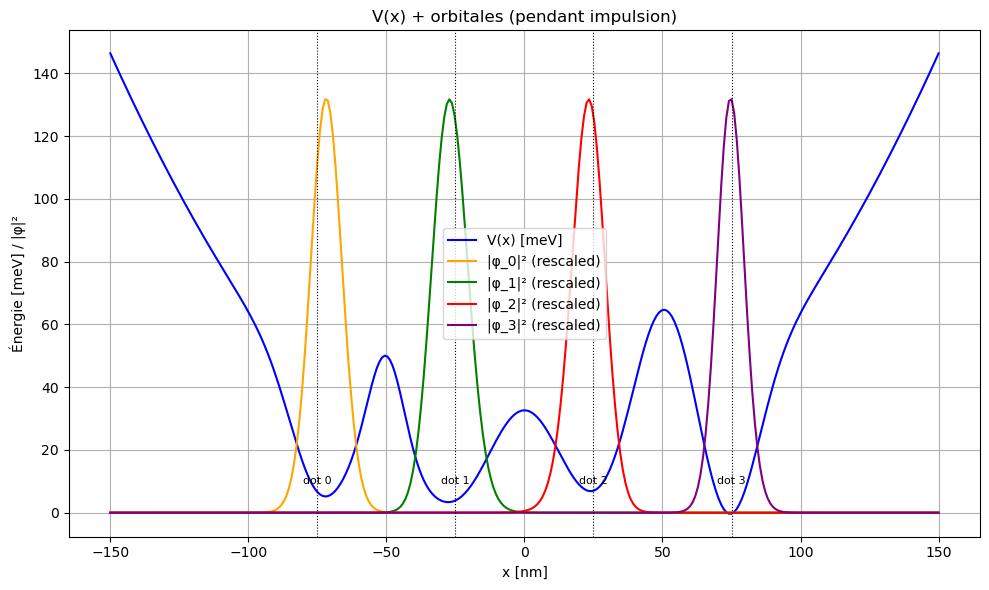
\includegraphics[width=\textwidth]{pdt_impulsion_bon.png}
    \subcaption{Vue 1D pendant impulsion}
    \label{fig:view_1D_on}
  \end{subfigure}

  \vspace{0.8em}

  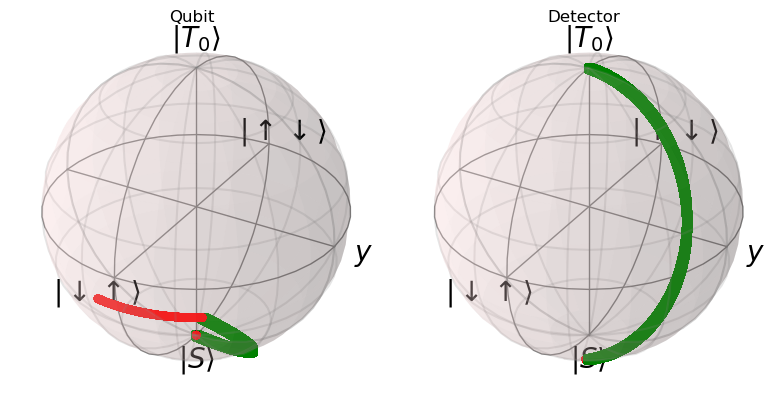
\includegraphics[width=0.6\textwidth]{singlet-triplet_du_57_dt_1_2_version1.png}

  \caption{Probabilité d'une détection idéale.}
  \label{fig:fidelity_map_detector}
\end{figure}

% --- Figure simple (1 image) ---
\begin{figure}[H]
  \centering
  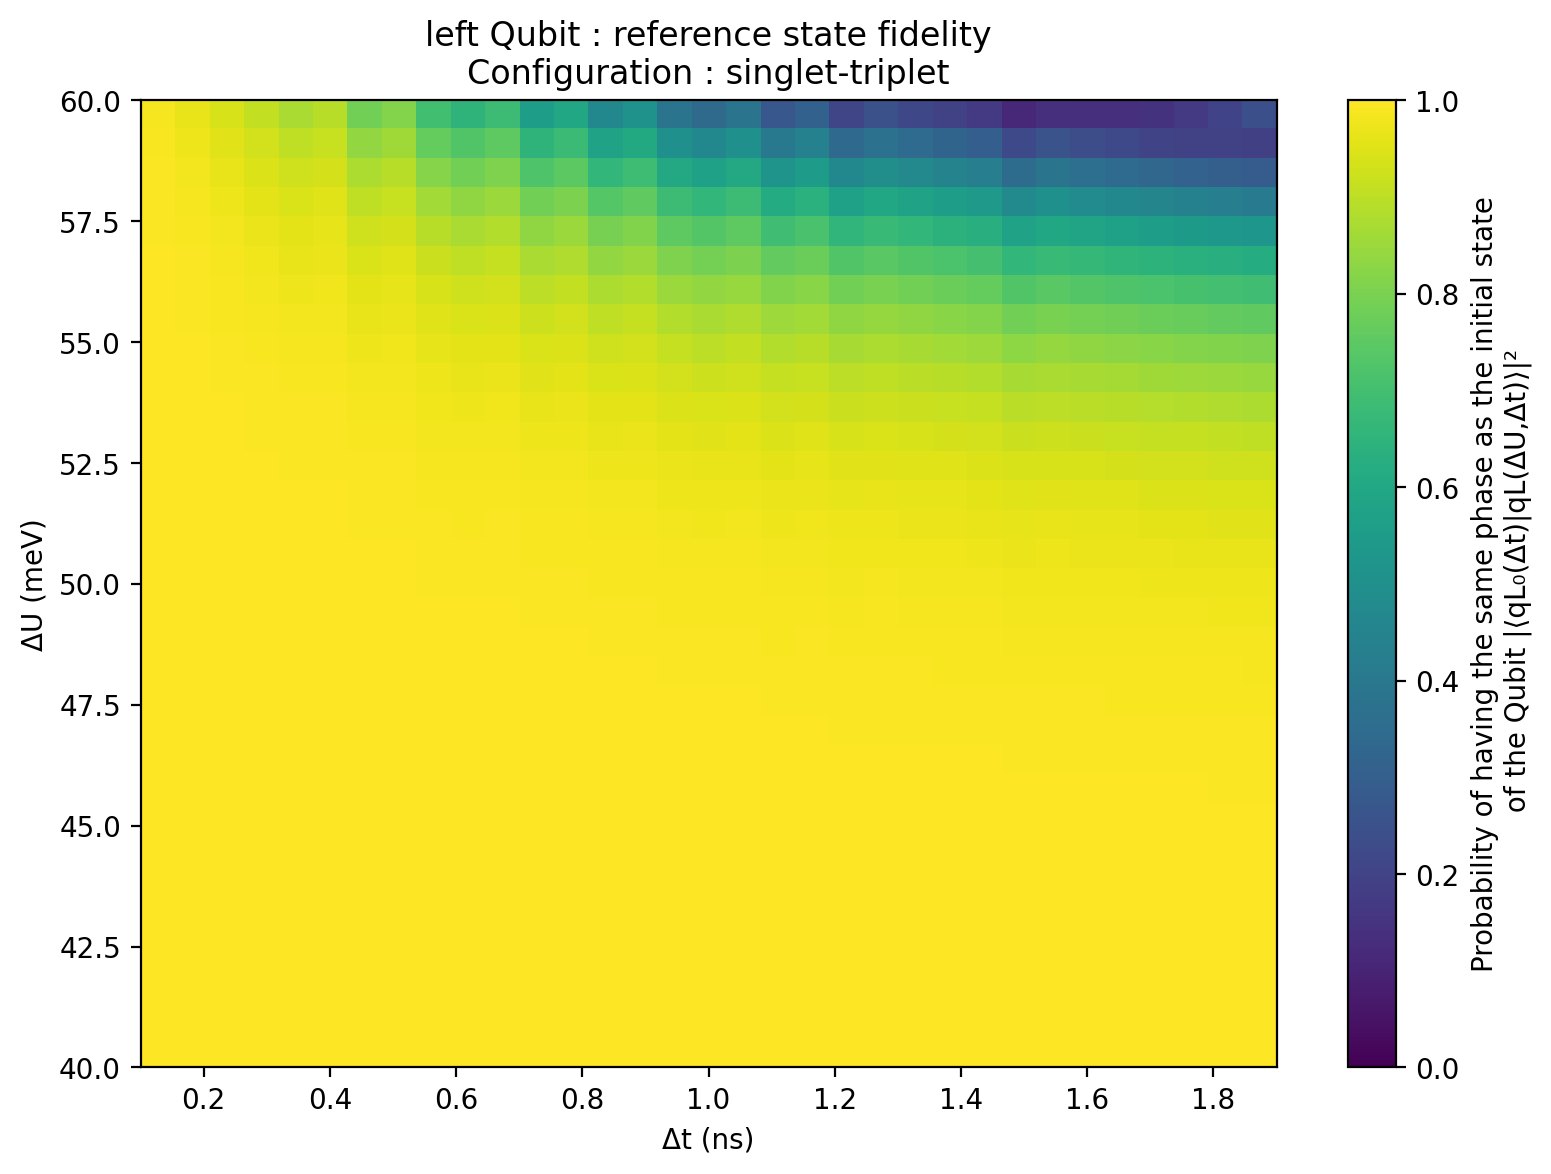
\includegraphics[width=0.6\textwidth]{p_qubit_overlap_map_left_33x33_20250822-064424.png}
  \caption{Carte de fidélité de la phase du détecteur.}
  \label{fig:fidelity_map_1}
\end{figure}


\subsection{Paramètres généraux :}
\begin{table}[H]
  \centering
  \caption{Paramètres de la simulation (issus de \texttt{param\_simu.py})}
  \label{tab:params}
  \begin{tabularx}{0.95\linewidth}{
      >{\raggedright\arraybackslash}p{4cm}
      >{\raggedright\arraybackslash}p{2.5cm}
      S[table-format=3.3]
      >{\raggedright\arraybackslash}X
  }
    \toprule
    \textbf{Symbole / Nom} & \textbf{Unité} & \textbf{Valeur} & \textbf{Description} \\
    \midrule
    $N_{\text{sites}}$       & — & 4 & Nombre de puits (dots) \\
    $N_{e}$                  & — & 4 & Nombre d’électrons \\
    $m_{\text{eff}}$         & $m_e$ & 0.067 & Masse effective (GaAs) \\
    $x_{\text{dots}}$        & \si{\nano\metre} & $\{-75,-25,25,75\}$ & Positions des 4 puits (x) \\
    $a$                      & \si{\milli\electronvolt\per\nano\metre\squared} & 6.5e-3 & Courbure du potentiel en $x$ \\
    Profondeurs puits        & \si{\milli\electronvolt} & (30, 5, 5, 40) & Énergies des 4 puits \\
    Hauteurs barrières       & \si{\milli\electronvolt} & (35, 90, 50) & Hauteurs des 3 barrières \\
    Largeur des puits        & \si{\nano\metre} & 23 & Largeur typique des puits \\
    Largeurs barrières       & \si{\nano\metre} & (15, 30, 25) & Largeurs des barrières \\
    $\sigma_x$               & \si{\nano\metre} & 15 & Largeur gaussienne en $x$ \\
    $\sigma_y$               & \si{\nano\metre} & 15 & Largeur gaussienne en $y$ (eff.) \\
    $y_{\text{confinement}}$ & \si{\milli\electronvolt\per\nano\metre\squared} & 0.1 & Confinement harmonique $y$ \\
    $t_{\text{imp}}$         & \si{\nano\second} & 0.1 & Instant de début de l’impulsion \\
    $\Delta t$               & \si{\nano\second} & 1.6 & Durée de l’impulsion \\
    $T_{\text{final}}$       & \si{\nano\second} & 2.0 & Temps total de simulation \\
    $\Delta U$               & \si{\milli\electronvolt} & 57 & Variation de $U$ due à l’impulsion \\
    $N_t$                    & — & 300 & Nombre de pas de temps \\
    $N_x$                    & — & dépend de la grille & Taille de la grille adaptative en $x$ \\
    $N_y$                    & — & dépend de la grille & Taille de la grille adaptative en $y$ \\
    \bottomrule
  \end{tabularx}
\end{table}


\end{document}
